\chapter{Dal RL al Deep RL}

\section{Reinforcement Learning}
Gli esseri umani per la maggior parte della loro vita sono immersi in un ambiente facendo esperienza dell'interazione con esso e registrando nel proprio cervello una grande quantità di informazioni rispetto a cause ed effetti, alle conseguenze delle proprie azioni e su come agire per raggiungere degli obiettivi.
Questa forma di insegnamento, che è l'interazione con l'ambiente in se, è in assoluto quella predominante nella vita degli individui, solo in piccola parte accompagnata da quello supervisionato.
Che si tratti di imparare a guidare o tenere una conversazione, siamo sempre molto attenti a come l'ambiente risponde alle nostre azioni con l'obiettivo di influenzare cosa succede attraverso esse.\cite{rlBook}\newline

Il Reinforcement Learning fonda le proprie basi teoriche ispirandosi proprio a questo aspetto del comportamento umano.\newline

Il Reinforcement Learning è la branca dell'Intelligenza Artificiale che si preoccupa di studiare il problema di un agente che deve apprendere un comportamento attraverso tentativi ed errori, interagendo con l'ambiente in cui è immerso.
Il tutto senza che gli venga specificato come agire ma solamente attraverso un meccanismo di ricompense e punizioni.\newline
\clearpage

\subsection{Il modello del RL}

Il modello standard del Reinforcement Learning è composto da un agente che è in comunicazione con un ambiente attraverso percezioni e azioni. Come si vede dalla fig.\ref{fig:rl_model}, in ogni istante di tempo $t$ l'agente riceve un insieme di percezioni $s_t$ e una ricompensa $r_t$ dall'ambiente e sceglie un'azione $a_t$ da eseguire. Tale azione cambia lo stato dell'ambiente, il quale emette una nuova ricompensa per l'agente.

\begin{figure}[hb]
    \centering
    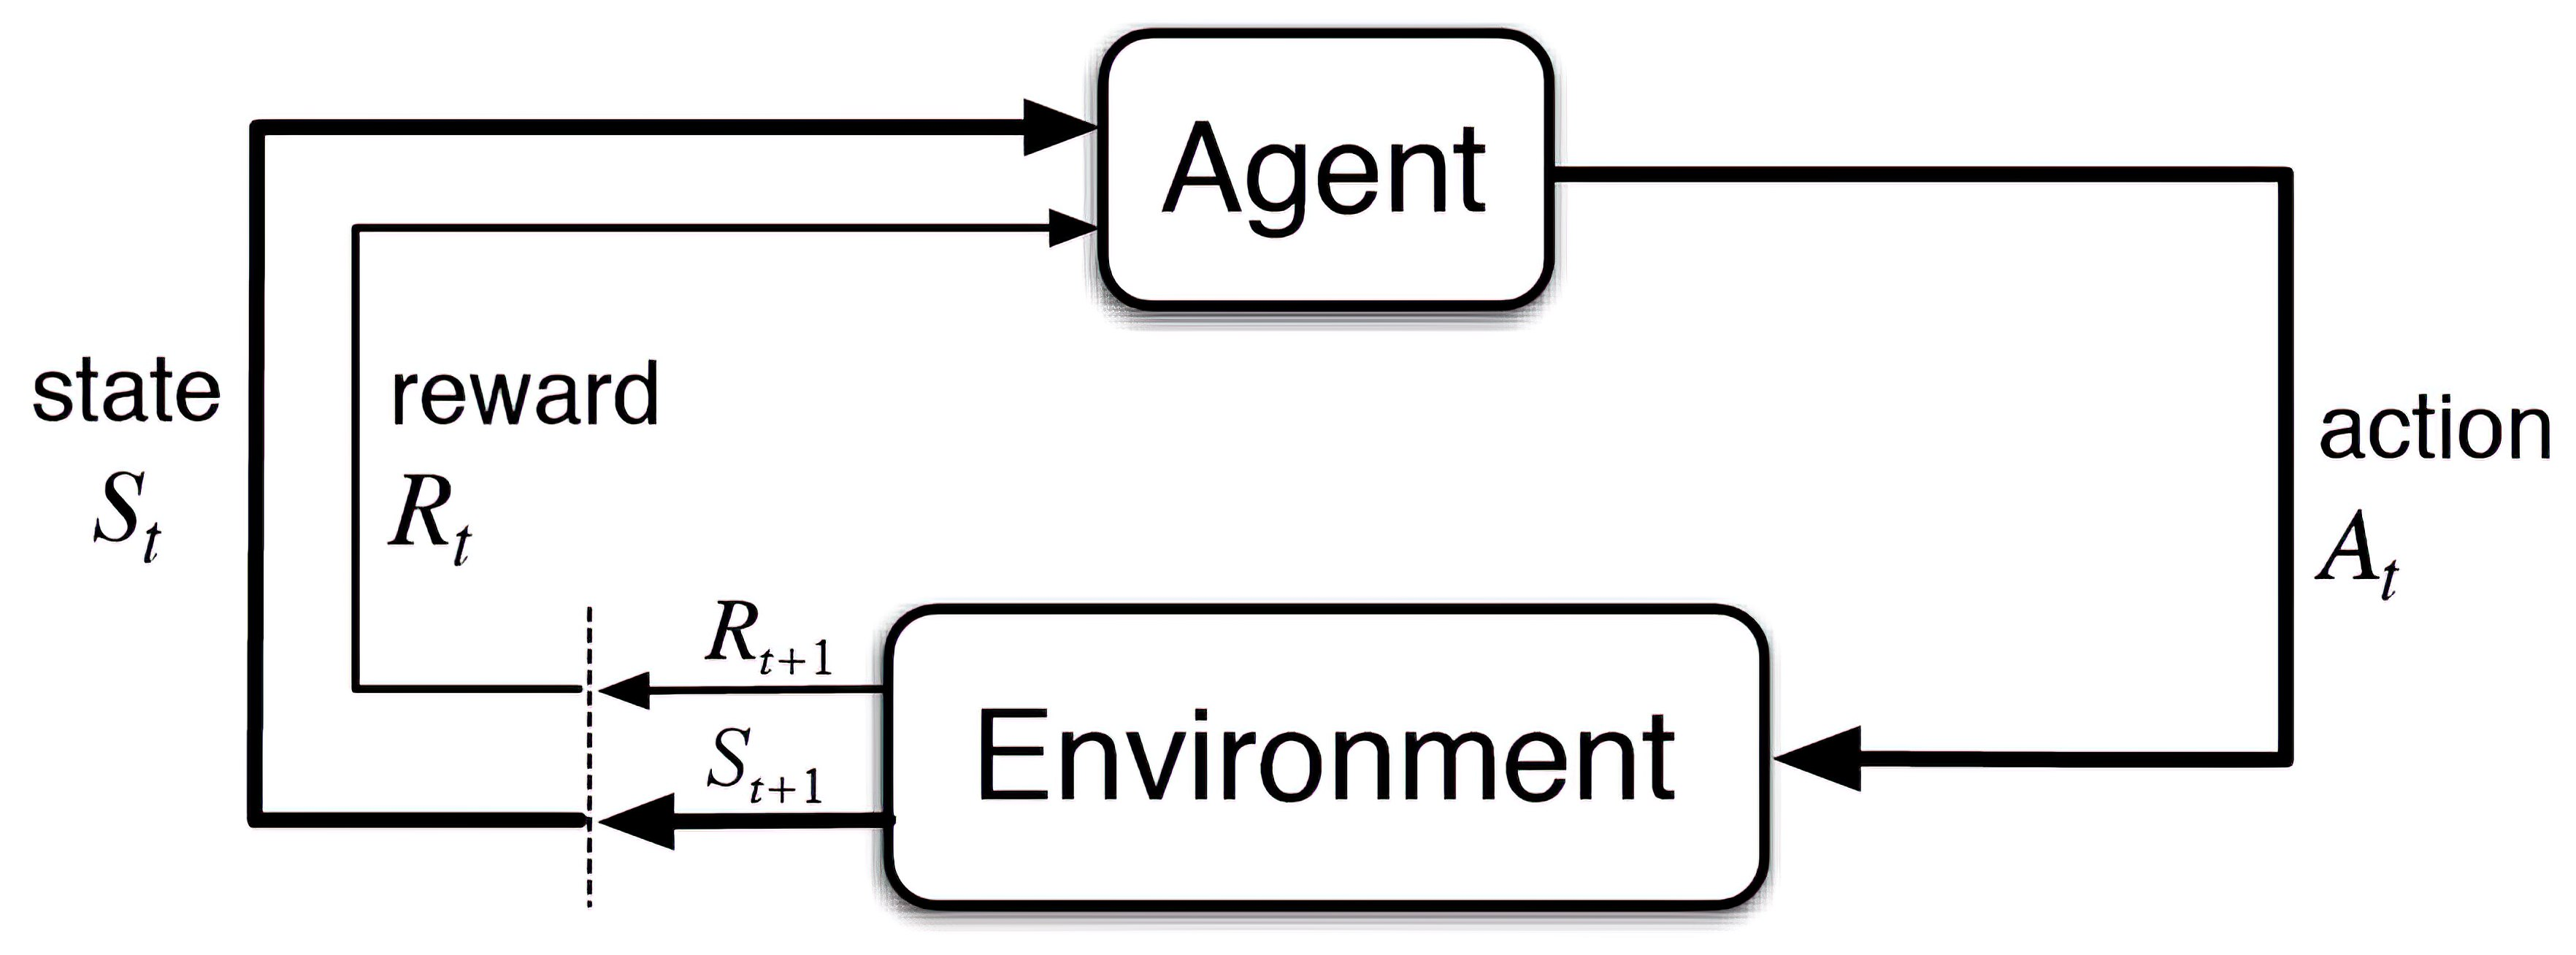
\includegraphics[width = 4in]{Figures/Chapter1/RL_model4x.jpg}
    \caption{Modello del RL}
    \label{fig:rl_model}
\end{figure}

La funzione che in ogni istante di tempo associa ad uno stato una distribuzione di probabilità sull'insieme delle azioni si chiama \textit{policy} e usualmente viene indicata col simbolo $\pi$.

\begin{equation}
	\pi: s \xrightarrow{} \mathcal{D}
\end{equation}

Per misurare la bontà di un'azione $a_t$ eseguita in uno stato $s_t$ viene definita la \textit{action-value function} $Q$ associata alla policy $\pi$

\begin{equation}\label{valueeq1}
	Q^\pi(s_t,a_t) = \mathbb{E}
	\Big[ 
	\sum\limits_{k = 0}^\infty\gamma^k \, r_{t+k}
	\Big]
\end{equation}

mentre per misurare il valore di uno stato $s_t$ si definisce la \textit{state-value function} $V$ associata alla policy $\pi$

\begin{equation}\label{valueev1}
	V^\pi(s_t) = \mathbb{E}
	\Big[ 
	\sum\limits_{k = 0}^\infty\gamma^k \, r_{t+k}
	\Big]
\end{equation}

Dove $\gamma \in [0,1]$ è chiamato \textit{discount factor} e controlla come l'agente valuta le ricompense future nell'ambito dei problemi ad orizzonte infinito\cite{rlSurvey}. Bassi valori favoriscono un comportamento teso a massimizzare le ricompense a breve termine mentre alti valori quelle a lungo termine.\newline

Q è calcolata come la media pesata rispetto a potenze di $\gamma$ delle ricompense future ottenute dall'agente in ottemperanza alla policy $\pi$. L'eq.\ref{valueeq1} è comunemente espressa nella forma di Bellman come segue

\begin{equation}
	Q^\pi(s_t,a_t) = r(s_t,a_t) + \gamma\, Q^\pi(s_{t+1},a_{t+1})
\end{equation}

Dove $r(s_t,a_t)$ è la ricompensa ottenuta nello stato di arrivo $s_{t+1}$ eseguendo l'azione $a_t$ nello stato $s_t$. Per tale motivo verrà indicata anche come $r_{t+1}$.\newline

La tupla $(s_t,a_t,s_{t+1},r_{t+1})$ viene detta \textit{transizione} e rappresenta l'unità fondamentale dell'apprendimento per gli algoritmi di RL nell'ambito dei \textit{Markov Decision Process}.

L'obiettivo dell'agente è imparare una \textit{policy ottima} $\pi^*$, a cui corrisponde una \textit{action-value function} ottima $Q^{\pi^*}$ che calcola il valore di ogni stato $s$ come la somma della ricompensa istantanea e del valore scontato dello stato successivo eseguendo \textit{la migliore azione possibile}

\begin{equation}\label{valueoptimaleq}
	Q^{\pi^*}(s_t,a_t) = r_{t+1} + \gamma \max_{a} Q^{\pi^*}(s_{t+1},a_{t+1}),\, \forall s
\end{equation}

Data la \ref{valueoptimaleq}, la policy ottima si determina come segue

\begin{equation}\label{qtopi}
	\pi^*(s_t) = \argmax_aQ^{\pi^*}(s_t,a_t)
\end{equation}

\clearpage

\subsection{Q-Learning}

Il Q-Learning\cite{qlearningPaper} è uno degli algoritmi model-free\footnote{Classe di algoritmi che non fa utilizzo del modello del processo da ottimizzare ma si basa sul trial-and-error.} più conosciuti del RL e fa parte della famiglia dei Temporal Difference\footnote{Famiglia di algoritmi basati su una ottimizzazione dinamica della stima della action-value function basata sulle osservazioni correnti.}. 

Il cuore dell'algoritmo, che usa la eq.\ref{valueeq1} come action value function, è la funzione di aggiornamento implementata dall'agente:

\begin{equation}
	Q(s_t,a_t) \xleftarrow{} Q(s_t,a_t) + 
	\alpha \,\Big[ r_{t+1} + \gamma\, \max_{a_{t+1}}Q(s_{t+1},a_{t+1}) - Q(s_t,a_t)\Big]
\end{equation}

Dove $\alpha \in [0,1]$ è il \textit{learning rate}, ovvero il tasso con il quale i valori di Q sono aggiornati ad ogni step, e $\gamma$ è quello definito in precedenza.
Sotto l'ipotesi che tutte le azioni sono campionate un numero sufficiente di volte in tutti gli stati e i valori stato-azione sono rappresentati in modo discreto si dimostra\cite{qlearningtecnicalPaper} che il Q-Learning converge con \textit{probabilità 1} alla action-value function ottima $Q^*$.

\clearpage

\section{Deep Reinforcement Learning}

Con l'evoluzione delle \textit{Deep Neural Network} è stato possibile rielaborare i classici algoritmi del RL e di formularne di nuovi. I benefici dell'utilizzo delle DNN come approssimatori di funzioni non lineari sono la possibilità di creare agenti più robusti alle variazioni ambientali e di gestire spazi di stato di dimensioni molto maggiori senza tante complicazioni sulla velocità computazionale.

\subsection{Metodi Value Based}

Questa famiglia di metodi si basa sulla stima della action-value function ottima $Q^*$ come base per poi ricavare una policy ottima $\pi^*$.

\subsubsection{Deep Q-Network}

Il DQN\cite{dqnPaper} è una variante del Q-Learning che implementa una DNN per approssimare la action-value function di eq.\ref{valueeq1}.
\newline

Come si vede dalla fig.\ref{fig:dqnnetwork} la rete riceve in ingresso lo stato attuale e presenta in uscita il \textit{valore} di ogni possibile azione.
Proprio per il fatto che il numero di neuroni in uscita ad una rete neurale non può essere infinito il DQN è utilizzabile solo nel caso di insiemi di azioni numerabili.

\begin{figure}[hb]
    \centering
    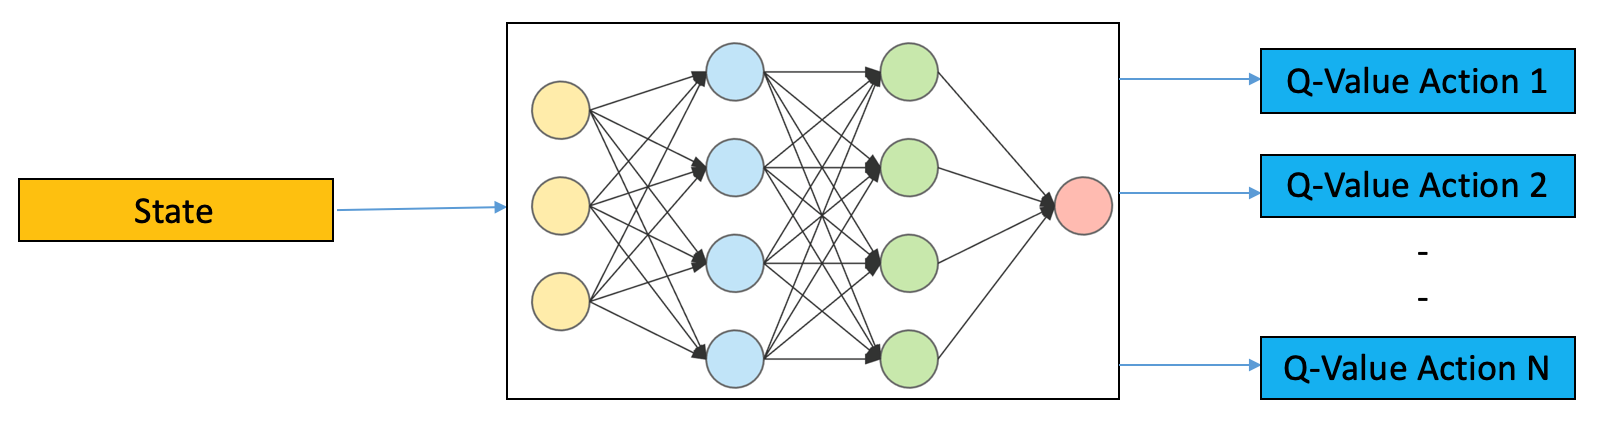
\includegraphics[width = 5.5in]{Figures/Chapter2/dqn.png}
    \caption{Topologia della Deep Q-Network}
    \label{fig:dqnnetwork}
\end{figure}

Per risolvere il problema della divergenza del RL nel caso di utilizzo di approssimatori di funzioni non lineari\cite{rlinstabilityPaper}, gli autori del DQN prevedono l'utilizzo di un \textit{experience replay}, ovvero un buffer dove vengono salvate le transizioni. L'obiettivo di tale aggiunta è che prelevando in maniera casuale le transizioni dal replay buffer si risolve il problema della correlazione tra la sequenza di osservazioni che è una delle cause della divergenza. 
\newline

Ad ogni time step $i$ si prelevano casualmente dall'experience replay un batch $D$ di transizioni e si aggiorna la rete Q seguendo il gradiente della \textit{loss function} di equazione:

\begin{equation}
L(\theta_i) = \mathbb{E}_D 
	\Bigg[ 
	\Big(
	r_{t+1} + \gamma\,\max_{a_{t+1}}Q(s_{t+1},a_{t+1} \,| \,\theta'_i) - Q(s_t,a_t \,| \, \theta_i)
	\Big)^2
	\Bigg]
\end{equation}
	

dove $Q(s_t,a_t \,| \, \theta_i)$ è la rete principale con parametri $\theta_i$ e $Q(s_{t+1},a_{t+1} \,| \,\theta'_i)$ è una seconda rete, detta \textit{target network}, che approssima la action-value function dello stato successivo. I suoi parametri $\theta'_i$ vengono aggiornati con una copia di quelli della main Q-network solo ogni $C$ iterazioni e mantenuti fissi tra gli aggiornamenti.

\clearpage

\subsection{Metodi Policy Based}

In opposizione ai metodi Value Based, questi mirano a stimare direttamente la policy ottima $\pi^*$. Possiamo categorizzarli in \textit{Stochastic Policy Based} o \textit{Deterministic Policy Based}. Il primo tipo di algoritmi produce una distribuzione di probabilità su un insieme numerabile di azioni, mentre il secondo determina direttamente il valore dell'azione da eseguire, e quindi è applicabile a processi con spazi di azioni continui.

\subsubsection{REINFORCE}

REINFORCE\cite{reinforcePaper} è un algoritmo Stochastic Policy Based che utilizza una DNN per implementare una policy $\pi$. Come si evince dalla fig.\ref{fig:reinforce} la rete produce una distribuzione di probabilità sull'insieme di azioni $[a_1,a_2,...,a_k]$ a partire da una osservazione $[s_1,s_2,...,s_N]$.
\newline

\begin{figure}[hb]
    \centering
    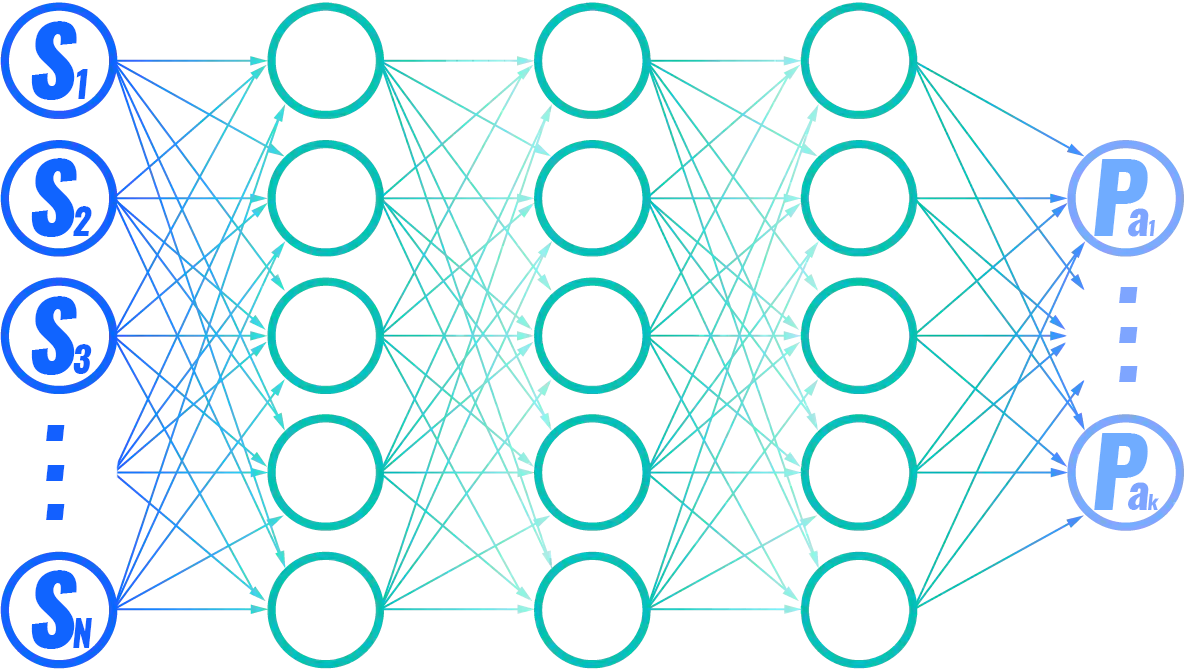
\includegraphics[width = 4in]{Figures/Chapter2/policy_network.png}
    \caption{Policy Network}
    \label{fig:reinforce}
\end{figure}

Il cuore dell'algoritmo è il processo di aggiornamento dei parametri $\theta$ della rete, che viene eseguito a fine di ogni \textit{episodio}\footnote{Un episodio è un insieme di step eseguiti dall'agente fino al raggiungimento di una delle possibili condizioni di terminazione prefissate.}, nella direzione del gradiente della funzione di performance $J(\theta)$ di eq:

\begin{equation}\label{reinforce_perf_eq}
	J(\theta) = \sum_{t=0}^{T-1} \gamma^t \, r_{t+1}
\end{equation}

dove T è il numero di step che compongono l'episodio e il gradiente ha eq:

\begin{equation}\label{reinforce_perf_grad_eq}
	\nabla_{\theta} J(\theta) = \sum_{t=0}^{T-1} \nabla_{\theta} \log \pi_{\theta}(a_t|s_t) \, G(t)
\end{equation}

con $G$ funzione di ricompensa cumulativa scontata di eq: 

\begin{equation}
	G(t) = \sum_{k=0}^{T-t-1} \gamma^k\,r_{t+k+1}
\end{equation}

Ulteriori dettagli sul processo di calcolo della eq.\ref{reinforce_perf_grad_eq} sono reperibili qui\cite{reinforcemathWebsite}.

\clearpage

\subsection{Metodi Actor-Critic}

Questi metodi sono un ibrido che combinano i benefici dei metodi Value Based e di quelli Policy Based. Consistono nell'utilizzo di due DNN, una per la stima della policy $\pi$, nominata \textit{Actor} e una per la stima della \textit{state value function} $V$, nominata \textit{Critic}. Nella fig.\ref{fig:actor-critic} si può osservare il modello.
\newline

\begin{figure}[hb]
    \centering
    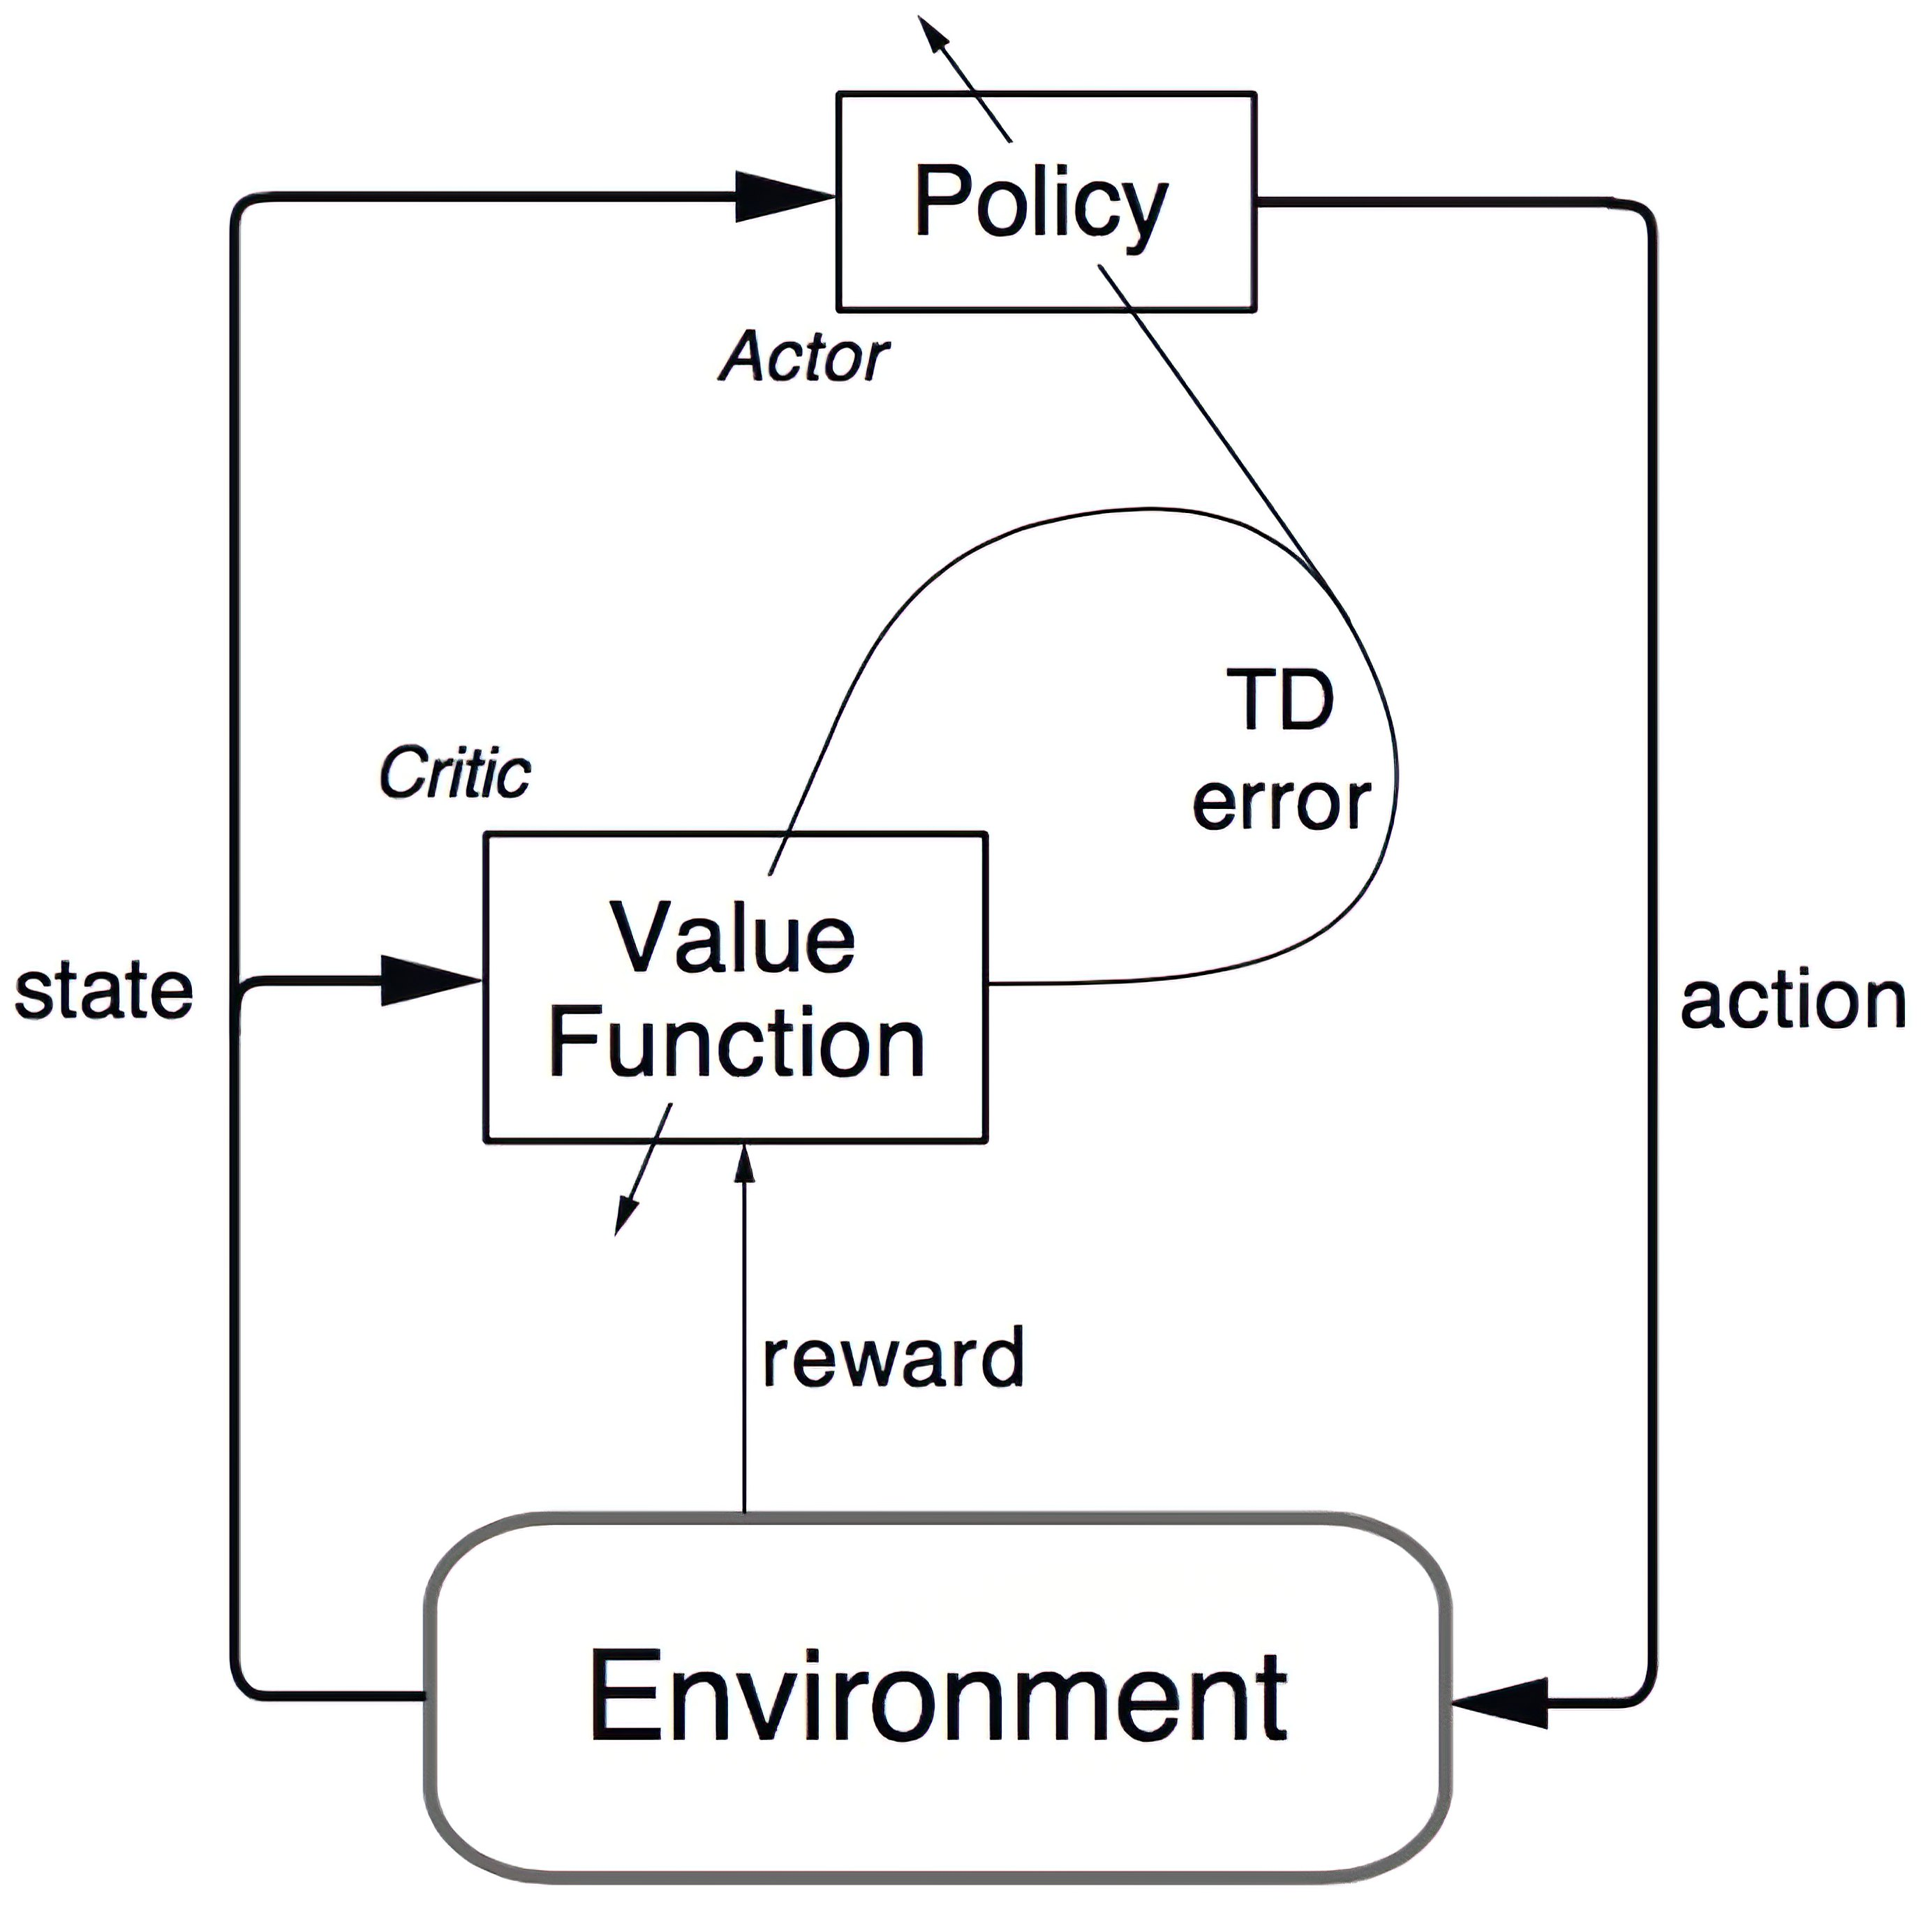
\includegraphics[width = 4in]{Figures/Chapter2/actor-critic_model4x.jpg}
    \caption{Modello dell'Actor-Critic}
    \label{fig:actor-critic}
\end{figure}

Ad ogni step $t$ dell'episodio l'Actor produce un'azione $a_t$ che modifica lo stato dell'ambiente. Il nuovo stato $s_{t+1}$ e la ricompensa associata $r_{t+1}$ vengono poi recepiti dal Critic che ne valuta la bontà attraverso la state-vale function $V_{\theta}(s_{t+1})$ di eq.\ref{valueev1}. Si tenga in considerazione che il Critic mantiene in memoria anche $V_{\theta}(s_t)$ derivante dallo stato precedente.
\newline

L'aggiornamento delle due reti viene fatto ogni step. I parametri $\theta$ della rete Critic vengono aggiornati nella direzione della minimizzazione della seguente funzione di costo:

\begin{equation}
	\delta^2 = \Big[ r_{t+1} + \gamma \, V_{\theta}(s_{t+1}) - V_{\theta}(s_t) \Big]^2
\end{equation}

mentre i parametri $\phi$ dell'Actor vengono aggiornati per minimizzare la funzione di costo:

\begin{equation}
	X = \delta \, \log \pi_{\phi}(a_t|s_t)
\end{equation}

\subsubsection{DDPG}\label{ddpgsection}

Il Deep Deterministic Policy Gradient (DDPG)\cite{ddpgPaper} è un algoritmo model-free e off-policy\footnote{Sono off-policy gli algoritmi che aggiornano i loro parametri basandosi su policy vecchie.}, facente parte della famiglia degli Actor-Critic, che permette ad un agente di imparare una Q-function e una policy \textit{specificatamente} in uno spazio di stato e di azione continuo.
\newline

Questo algoritmo è strettamente connesso al Q-learning ed è motivato allo stesso modo: se si conosce la action-value function ottima $Q^*(s,a)$ allora, in ogni dato stato, la policy ottima può essere trovata risolvendo l'eq.\ref{qtopi}.
\newline

Quando c'è un numero finito di azioni, il calcolo del massimo non pone problemi perché si possono calcolare i Q-value per ogni azione separatamente e successivamente confrontarli. Ma quando lo spazio delle azioni è continuo, non è possibile valutare in modo esauriente il massimo tra i Q-value in quanto si sarebbe costretti a campionare lo spazio d'azione e questo porterebbe inevitabilmente ad errori di valutazione. Inoltre l'utilizzo di un normale algoritmo di calcolo del massimo renderebbe la subroutine estremamente inefficiente all'aumentare del numero delle azioni.
\newline

Tuttavia poiché lo spazio delle azioni è continuo, si presume che la funzione $Q^*(s,a)$ sia differenziabile rispetto all'azione $a$. Questo consente di impostare un apprendimento basato sul gradiente per una policy $\mu(s)$. Quindi, invece di eseguire una costosa subroutine di ottimizzazione ogni volta che si desidera calcolare $\max_{a} Q(s,a)$, è possibile approssimarlo con $Q(s,\mu(s))$.
\newline

Il modello prevede l'utilizzo di due coppie di DNN: 
\begin{itemize}
    \item Una coppia di reti principali: $\mu_{\phi}(s)$, chiamata Actor, che sarà utilizzata per stimare la policy ottima e $Q_{\theta}(s,a)$, chiamata Critic, che stimerà la action-value function ottima.
\item Una seconda coppia di reti: $\mu_{\phi_{targ}}(s)$ e $Q_{\theta_{targ}}(s,a)$, dette \textit{Target Actor} e \textit{Target Critic}, che saranno utilizzate per il calcolo della loss function che permetterà l'aggiornamento dei parametri delle prime due. Queste reti hanno la stessa struttura di quelle principali e vengono aggiornate periodicamente attraverso un \textit{soft update} in base ai loro parametri.
\end{itemize}

Le reti target vengono adoperate in modo che il valore atteso target non sia dipendente dai parametri utilizzati nelle reti principali che calcolano il valore atteso attuale. In questo modo si evitano grosse divergenze tra i due valori migliorando la stabilità durante l’addestramento. Come nel DQN, il DDPG utilizza un experience replay per campionare le esperienze passate e aggiornare i parametri della rete neurale.
\newline

Dato un insieme $D$ di transizioni prelevate dall'experience replay, l'aggiornamento dei parametri della $Q_{\theta}(s,a)$ viene fatta nella direzione di minimizzazione del mean-squared Bellman error (MSBE), che quantifica in che misura $Q_{\theta}$ si avvicina a soddisfare l'equazione di Bellman:

\begin{equation}\label{criticlossddpg}
  L(\theta) = \mathbb{E}_D 
	\Bigg[ 
	\bigg(
	Q_{\theta}(s_t,a_t) - 
	\Big(
	r_{t+1} + \gamma(1-d)Q_{\theta_{targ}}(s_{t+1},\mu_{\phi_{targ}}(s_{t+1}))
	\Big)
	\bigg)^2
	\Bigg]  
\end{equation}

con $d$ un flag booleano posto ad 1 quando $s_{t+1}$ è uno stato terminale, in modo che la Q-function non attribuisca ulteriore valore all'azione se non quella conferita dalla ricompensa immediata $r_{t+1}$.
\newline

L'aggiornamento dei parametri dell'Actor è più intuitivo in quanto viene fatto seguendo la massimizzazione della funzione $Q_{\theta}(s_t,\mu_{\phi}(s))$ rispetto i sui parametri $\phi$, e quindi nella direzione del gradiente:

\begin{equation}\label{gradactorddpg}
   \nabla_{\phi} \, Q_{\theta}(s_t,\mu_{\phi}(s)) =
   \frac{\partial}{\partial \mu_{\phi}} \, Q_{\theta}(s_t,\mu_{\phi}(s)) \,
   \frac{\partial}{\partial\phi} \, \mu_{\phi}(s)
\end{equation}


I parametri delle reti target vengono aggiornati seguendo un \textit{soft update}:

\begin{equation}\label{ddpgsoftupdate_eq}
   \begin{aligned}
       &\theta_{targ} \xleftarrow{} \tau \theta + (1-\tau) \theta_{targ} \\
       &\phi_{targ} \xleftarrow{} \tau \phi + (1-\tau) \phi_{targ}
   \end{aligned}
\end{equation}

dove $\tau$ è detto \textit{smooth factor} e generalmente è molto piccolo per garantire un aggiornamento lento delle reti target.

\clearpage

Di seguito viene mostrato lo pseudocodice dell'algoritmo DDPG\cite{ddpgPaper}:

\begin{figure}[hb]
    \centering
    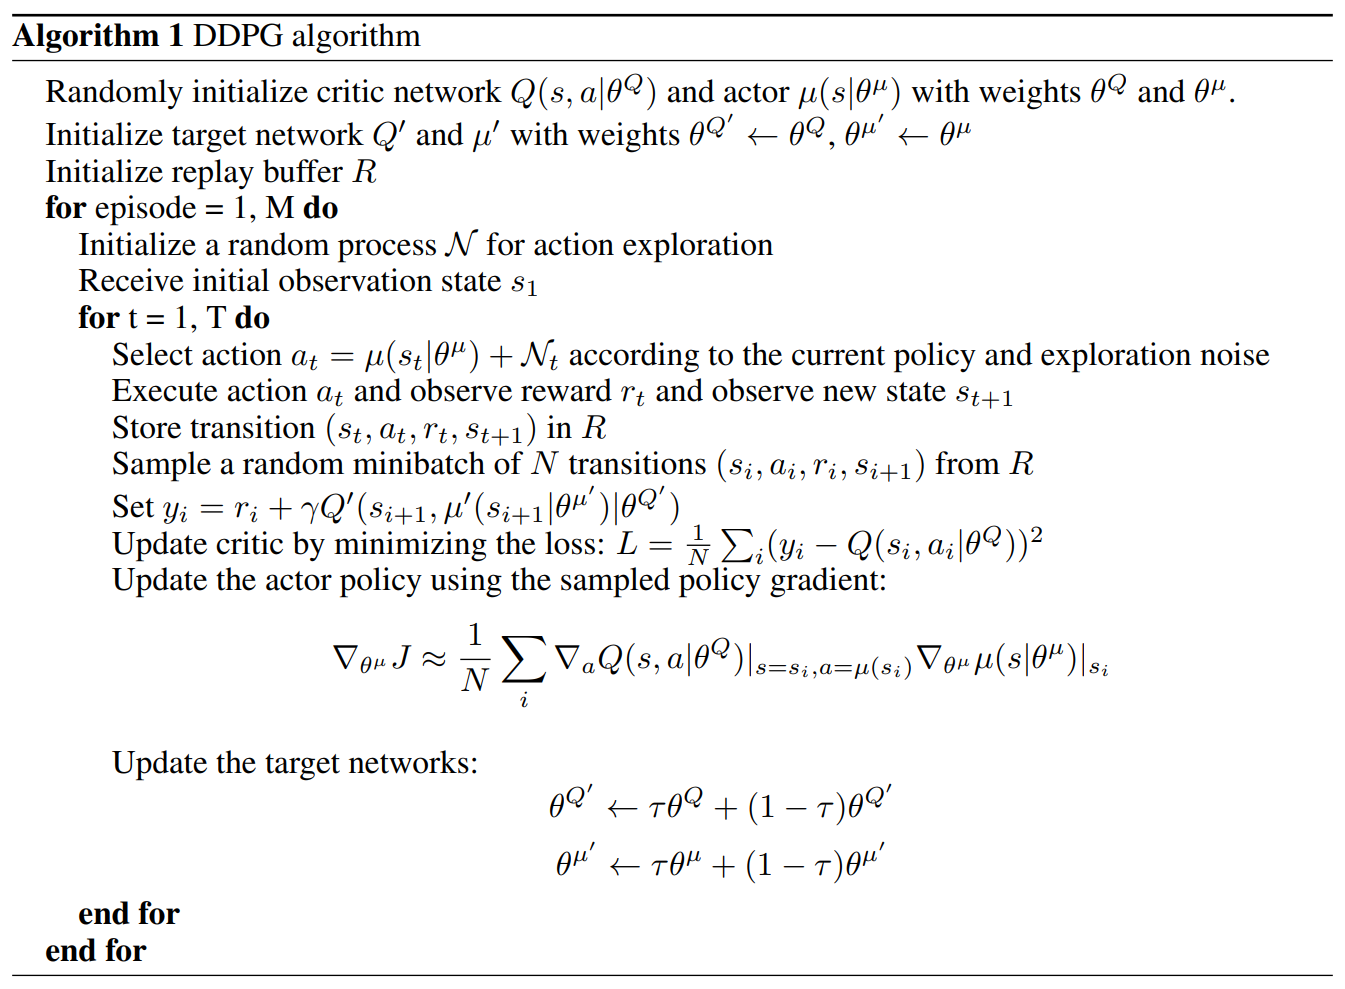
\includegraphics[width = 6in]{Figures/Chapter2/ddpg_algo.png}
    \caption{Algoritmo DDPG}
    \label{fig:ddpgalgo}
\end{figure}

\clearpage